\documentclass[]{book}
\usepackage{lmodern}
\usepackage{amssymb,amsmath}
\usepackage{ifxetex,ifluatex}
\usepackage{fixltx2e} % provides \textsubscript
\ifnum 0\ifxetex 1\fi\ifluatex 1\fi=0 % if pdftex
  \usepackage[T1]{fontenc}
  \usepackage[utf8]{inputenc}
\else % if luatex or xelatex
  \ifxetex
    \usepackage{mathspec}
  \else
    \usepackage{fontspec}
  \fi
  \defaultfontfeatures{Ligatures=TeX,Scale=MatchLowercase}
\fi
% use upquote if available, for straight quotes in verbatim environments
\IfFileExists{upquote.sty}{\usepackage{upquote}}{}
% use microtype if available
\IfFileExists{microtype.sty}{%
\usepackage{microtype}
\UseMicrotypeSet[protrusion]{basicmath} % disable protrusion for tt fonts
}{}
\usepackage[margin=1in]{geometry}
\usepackage{hyperref}
\hypersetup{unicode=true,
            pdftitle={MATH 697},
            pdfauthor={Sahir Rai Bhatnagar},
            pdfborder={0 0 0},
            breaklinks=true}
\urlstyle{same}  % don't use monospace font for urls
\usepackage{natbib}
\bibliographystyle{apalike}
\usepackage{color}
\usepackage{fancyvrb}
\newcommand{\VerbBar}{|}
\newcommand{\VERB}{\Verb[commandchars=\\\{\}]}
\DefineVerbatimEnvironment{Highlighting}{Verbatim}{commandchars=\\\{\}}
% Add ',fontsize=\small' for more characters per line
\usepackage{framed}
\definecolor{shadecolor}{RGB}{248,248,248}
\newenvironment{Shaded}{\begin{snugshade}}{\end{snugshade}}
\newcommand{\KeywordTok}[1]{\textcolor[rgb]{0.13,0.29,0.53}{\textbf{#1}}}
\newcommand{\DataTypeTok}[1]{\textcolor[rgb]{0.13,0.29,0.53}{#1}}
\newcommand{\DecValTok}[1]{\textcolor[rgb]{0.00,0.00,0.81}{#1}}
\newcommand{\BaseNTok}[1]{\textcolor[rgb]{0.00,0.00,0.81}{#1}}
\newcommand{\FloatTok}[1]{\textcolor[rgb]{0.00,0.00,0.81}{#1}}
\newcommand{\ConstantTok}[1]{\textcolor[rgb]{0.00,0.00,0.00}{#1}}
\newcommand{\CharTok}[1]{\textcolor[rgb]{0.31,0.60,0.02}{#1}}
\newcommand{\SpecialCharTok}[1]{\textcolor[rgb]{0.00,0.00,0.00}{#1}}
\newcommand{\StringTok}[1]{\textcolor[rgb]{0.31,0.60,0.02}{#1}}
\newcommand{\VerbatimStringTok}[1]{\textcolor[rgb]{0.31,0.60,0.02}{#1}}
\newcommand{\SpecialStringTok}[1]{\textcolor[rgb]{0.31,0.60,0.02}{#1}}
\newcommand{\ImportTok}[1]{#1}
\newcommand{\CommentTok}[1]{\textcolor[rgb]{0.56,0.35,0.01}{\textit{#1}}}
\newcommand{\DocumentationTok}[1]{\textcolor[rgb]{0.56,0.35,0.01}{\textbf{\textit{#1}}}}
\newcommand{\AnnotationTok}[1]{\textcolor[rgb]{0.56,0.35,0.01}{\textbf{\textit{#1}}}}
\newcommand{\CommentVarTok}[1]{\textcolor[rgb]{0.56,0.35,0.01}{\textbf{\textit{#1}}}}
\newcommand{\OtherTok}[1]{\textcolor[rgb]{0.56,0.35,0.01}{#1}}
\newcommand{\FunctionTok}[1]{\textcolor[rgb]{0.00,0.00,0.00}{#1}}
\newcommand{\VariableTok}[1]{\textcolor[rgb]{0.00,0.00,0.00}{#1}}
\newcommand{\ControlFlowTok}[1]{\textcolor[rgb]{0.13,0.29,0.53}{\textbf{#1}}}
\newcommand{\OperatorTok}[1]{\textcolor[rgb]{0.81,0.36,0.00}{\textbf{#1}}}
\newcommand{\BuiltInTok}[1]{#1}
\newcommand{\ExtensionTok}[1]{#1}
\newcommand{\PreprocessorTok}[1]{\textcolor[rgb]{0.56,0.35,0.01}{\textit{#1}}}
\newcommand{\AttributeTok}[1]{\textcolor[rgb]{0.77,0.63,0.00}{#1}}
\newcommand{\RegionMarkerTok}[1]{#1}
\newcommand{\InformationTok}[1]{\textcolor[rgb]{0.56,0.35,0.01}{\textbf{\textit{#1}}}}
\newcommand{\WarningTok}[1]{\textcolor[rgb]{0.56,0.35,0.01}{\textbf{\textit{#1}}}}
\newcommand{\AlertTok}[1]{\textcolor[rgb]{0.94,0.16,0.16}{#1}}
\newcommand{\ErrorTok}[1]{\textcolor[rgb]{0.64,0.00,0.00}{\textbf{#1}}}
\newcommand{\NormalTok}[1]{#1}
\usepackage{longtable,booktabs}
\usepackage{graphicx,grffile}
\makeatletter
\def\maxwidth{\ifdim\Gin@nat@width>\linewidth\linewidth\else\Gin@nat@width\fi}
\def\maxheight{\ifdim\Gin@nat@height>\textheight\textheight\else\Gin@nat@height\fi}
\makeatother
% Scale images if necessary, so that they will not overflow the page
% margins by default, and it is still possible to overwrite the defaults
% using explicit options in \includegraphics[width, height, ...]{}
\setkeys{Gin}{width=\maxwidth,height=\maxheight,keepaspectratio}
\IfFileExists{parskip.sty}{%
\usepackage{parskip}
}{% else
\setlength{\parindent}{0pt}
\setlength{\parskip}{6pt plus 2pt minus 1pt}
}
\setlength{\emergencystretch}{3em}  % prevent overfull lines
\providecommand{\tightlist}{%
  \setlength{\itemsep}{0pt}\setlength{\parskip}{0pt}}
\setcounter{secnumdepth}{5}
% Redefines (sub)paragraphs to behave more like sections
\ifx\paragraph\undefined\else
\let\oldparagraph\paragraph
\renewcommand{\paragraph}[1]{\oldparagraph{#1}\mbox{}}
\fi
\ifx\subparagraph\undefined\else
\let\oldsubparagraph\subparagraph
\renewcommand{\subparagraph}[1]{\oldsubparagraph{#1}\mbox{}}
\fi

%%% Use protect on footnotes to avoid problems with footnotes in titles
\let\rmarkdownfootnote\footnote%
\def\footnote{\protect\rmarkdownfootnote}

%%% Change title format to be more compact
\usepackage{titling}

% Create subtitle command for use in maketitle
\newcommand{\subtitle}[1]{
  \posttitle{
    \begin{center}\large#1\end{center}
    }
}

\setlength{\droptitle}{-2em}
  \title{MATH 697}
  \pretitle{\vspace{\droptitle}\centering\huge}
  \posttitle{\par}
  \author{Sahir Rai Bhatnagar}
  \preauthor{\centering\large\emph}
  \postauthor{\par}
  \predate{\centering\large\emph}
  \postdate{\par}
  \date{2017-08-17}

\usepackage{booktabs}
\usepackage{longtable}
\usepackage[bf,singlelinecheck=off]{caption}

%\usepackage{fontspec}
%\setmainfont[UprightFeatures={SmallCapsFont=AlegreyaSC-Regular}]{Alegreya}

\usepackage{framed,color}
\definecolor{shadecolor}{RGB}{248,248,248}

\renewcommand{\textfraction}{0.05}
\renewcommand{\topfraction}{0.8}
\renewcommand{\bottomfraction}{0.8}
\renewcommand{\floatpagefraction}{0.75}

%\renewenvironment{quote}{\begin{VF}}{\end{VF}}
%\let\oldhref\href
%\renewcommand{\href}[2]{#2\footnote{\url{#1}}}

\ifxetex
  \usepackage{letltxmacro}
  \setlength{\XeTeXLinkMargin}{1pt}
  \LetLtxMacro\SavedIncludeGraphics\includegraphics
  \def\includegraphics#1#{% #1 catches optional stuff (star/opt. arg.)
    \IncludeGraphicsAux{#1}%
  }%
  \newcommand*{\IncludeGraphicsAux}[2]{%
    \XeTeXLinkBox{%
      \SavedIncludeGraphics#1{#2}%
    }%
  }%
\fi

\makeatletter
\newenvironment{kframe}{%
\medskip{}
\setlength{\fboxsep}{.8em}
 \def\at@end@of@kframe{}%
 \ifinner\ifhmode%
  \def\at@end@of@kframe{\end{minipage}}%
  \begin{minipage}{\columnwidth}%
 \fi\fi%
 \def\FrameCommand##1{\hskip\@totalleftmargin \hskip-\fboxsep
 \colorbox{shadecolor}{##1}\hskip-\fboxsep
     % There is no \\@totalrightmargin, so:
     \hskip-\linewidth \hskip-\@totalleftmargin \hskip\columnwidth}%
 \MakeFramed {\advance\hsize-\width
   \@totalleftmargin\z@ \linewidth\hsize
   \@setminipage}}%
 {\par\unskip\endMakeFramed%
 \at@end@of@kframe}
\makeatother

\renewenvironment{Shaded}{\begin{kframe}}{\end{kframe}}

\newenvironment{rmdblock}[1]
  {
  \begin{itemize}
  \renewcommand{\labelitemi}{
    \raisebox{-.7\height}[0pt][0pt]{
      {\setkeys{Gin}{width=3em,keepaspectratio}\includegraphics{images/#1}}
    }
  }
  \setlength{\fboxsep}{1em}
  \begin{kframe}
  \item
  }
  {
  \end{kframe}
  \end{itemize}
  }
\newenvironment{rmdnote}
  {\begin{rmdblock}{note}}
  {\end{rmdblock}}
\newenvironment{rmdcaution}
  {\begin{rmdblock}{caution}}
  {\end{rmdblock}}
\newenvironment{rmdimportant}
  {\begin{rmdblock}{important}}
  {\end{rmdblock}}
\newenvironment{rmdtip}
  {\begin{rmdblock}{tip}}
  {\end{rmdblock}}
\newenvironment{rmdwarning}
  {\begin{rmdblock}{warning}}
  {\end{rmdblock}}

\usepackage{makeidx}
\makeindex

\urlstyle{tt}

\usepackage{amsthm}
\makeatletter
\def\thm@space@setup{%
  \thm@preskip=8pt plus 2pt minus 4pt
  \thm@postskip=\thm@preskip
}
\makeatother

%\usepackage[pagebackref=false,bookmarks]{hyperref}
\hypersetup{
	unicode=false,          
	pdftoolbar=true,        
	pdfmenubar=true,        
	pdffitwindow=false,     % window fit to page when opened
	pdfstartview={FitH},    % fits the width of the page to the window
	pdftitle={Manuscript 1},    % title
	pdfauthor={Sahir Rai Bhatnagar},     % author
	pdfsubject={Subject},   % subject of the document
	pdfcreator={Sahir Rai Bhatnagar},   % creator of the document
	pdfproducer={Sahir Rai Bhatnagar}, % producer of the document
	pdfkeywords={}, % list of keywords
	pdfnewwindow=true,      % links in new window
	colorlinks=true,       % false: boxed links; true: colored links
	linkcolor=red,          % color of internal links (change box color with linkbordercolor)
	citecolor=blue,        % color of links to bibliography
	filecolor=black,      % color of file links
	urlcolor=cyan           % color of external links
}


%\frontmatter % turns off chapter numbering and uses roman numerals for page numbers;
% https://tex.stackexchange.com/questions/20538/what-is-the-right-order-when-using-frontmatter-tableofcontents-mainmatter

\usepackage{amsthm}
\newtheorem{theorem}{Theorem}[chapter]
\newtheorem{lemma}{Lemma}[chapter]
\theoremstyle{definition}
\newtheorem{definition}{Definition}[chapter]
\newtheorem{corollary}{Corollary}[chapter]
\newtheorem{proposition}{Proposition}[chapter]
\theoremstyle{definition}
\newtheorem{example}{Example}[chapter]
\theoremstyle{remark}
\newtheorem*{remark}{Remark}
\let\BeginKnitrBlock\begin \let\EndKnitrBlock\end
\begin{document}
\maketitle

{
\setcounter{tocdepth}{1}
\tableofcontents
}
\chapter*{Syllabus}\label{syllabus}
\addcontentsline{toc}{chapter}{Syllabus}

\section*{General Information}\label{general-information}
\addcontentsline{toc}{section}{General Information}

\begin{itemize}
\tightlist
\item
  Instructor: Sahir Bhatnagar
\item
  Email:
  \href{mailto:sahir.bhatnagar@mail.mcgill.ca}{\nolinkurl{sahir.bhatnagar@mail.mcgill.ca}}
\item
  Website: \url{http://sahirbhatnagar.com/MATH697/}
\item
  Lectures: Tuesdays 9am - 12pm
\item
  Office: TBD
\item
  Office Hours: By appointment only
\item
  Prerequisite(s): Calculus and Algebra
\item
  Texts: \emph{Modern Mathematical Statistics with Applications}, 2nd
  Edition by Jay L. Devore and Kenneth N. Berk
\end{itemize}

\section*{Course Description}\label{course-description}
\addcontentsline{toc}{section}{Course Description}

The main learning outcomes of this course are to get a broad idea about
some frequently used probability models and to learn basic results and
techniques in probability theory and statistical inference. Most of the
materials for the course will be drawn from the first seven chapters of
the textbook. The book does not, however, contain all the materials we
intend to cover in this course. Some extra notes will therefore be given
on those topics not in the text book. We will also introduce
computational methods in statistics with the statistical software
program \texttt{R}.

\section*{Grade Distribution}\label{grade-distribution}
\addcontentsline{toc}{section}{Grade Distribution}

\begin{tabular}{l|l}
\hline
 & \\
\hline
Assignments & 10\%\\
\hline
Quizzes & 40\%\\
\hline
Final Exam & 50\%\\
\hline
\end{tabular}

\section*{Target Syllabus}\label{target-syllabus}
\addcontentsline{toc}{section}{Target Syllabus}

\subsection*{Overview and Descriptive Statistics (Weeks
1-4)}\label{overview-and-descriptive-statistics-weeks-1-4}
\addcontentsline{toc}{subsection}{Overview and Descriptive Statistics
(Weeks 1-4)}

\begin{itemize}
\tightlist
\item
  1.1 Populations and Samples
\item
  1.2 Pictorial and Tabular Methods in Descriptive Statistics
\item
  1.3 Measures of Location
\item
  1.4 Measures of Variability
\end{itemize}

\subsection*{Probability (Weeks 1-4)}\label{probability-weeks-1-4}
\addcontentsline{toc}{subsection}{Probability (Weeks 1-4)}

\begin{itemize}
\tightlist
\item
  2.1 Sample Spaces and Events
\item
  2.2 Axioms, Interpretations, and Properties of Probability
\item
  2.3 Counting Techniques
\item
  2.4 Conditional Probability
\item
  2.5 Independence
\end{itemize}

\subsection*{Discrete Random Variables and Probability Distributions
(Weeks
1-4)}\label{discrete-random-variables-and-probability-distributions-weeks-1-4}
\addcontentsline{toc}{subsection}{Discrete Random Variables and
Probability Distributions (Weeks 1-4)}

\begin{itemize}
\tightlist
\item
  3.1 Random Variables
\item
  3.2 Probability Distributions for Discrete Random Variables
\item
  3.3 Expected Values of Discrete Random Variables
\item
  3.4 Moments and Moment Generating Functions
\item
  3.5 The Binomial Probability Distribution
\item
  3.7 The Poisson Probability Distribution
\end{itemize}

\subsection*{Continuous Random Variables and Probability Distributions
(Weeks
5-8)}\label{continuous-random-variables-and-probability-distributions-weeks-5-8}
\addcontentsline{toc}{subsection}{Continuous Random Variables and
Probability Distributions (Weeks 5-8)}

\begin{itemize}
\tightlist
\item
  4.1 Probability Density Functions and Cumulative Distribution
  Functions
\item
  4.2 Expected Values and Moment Generating Functions
\item
  4.3 The Normal Distribution
\item
  4.7 Transformations of a Random Variable
\end{itemize}

\subsection*{Joint Probability Distributions (Weeks
5-8)}\label{joint-probability-distributions-weeks-5-8}
\addcontentsline{toc}{subsection}{Joint Probability Distributions (Weeks
5-8)}

\begin{itemize}
\tightlist
\item
  5.1 Jointly Distributed Random Variables
\item
  5.2 Expected Values, Covariance, and Correlation
\item
  5.3 Conditional Distributions
\item
  5.4 Transformations of Random Variables
\end{itemize}

\subsection*{Statistics and Sampling Distributions (Weeks
5-8)}\label{statistics-and-sampling-distributions-weeks-5-8}
\addcontentsline{toc}{subsection}{Statistics and Sampling Distributions
(Weeks 5-8)}

\begin{itemize}
\tightlist
\item
  6.1 Statistics and Their Distributions
\item
  6.2 The Distribution of the Sample Mean
\item
  6.3 The Mean, Variance, and MGF for Several Variables
\item
  6.4 Distributions Based on a Normal Random Sample
\end{itemize}

\subsection*{Point Estimation (Weeks
9-12)}\label{point-estimation-weeks-9-12}
\addcontentsline{toc}{subsection}{Point Estimation (Weeks 9-12)}

\begin{itemize}
\tightlist
\item
  7.1 General Concepts and Criteria
\item
  7.2 Methods of Point Estimation
\end{itemize}

\subsection*{Statistical Intervals Based on a Single Sample (Weeks
9-12)}\label{statistical-intervals-based-on-a-single-sample-weeks-9-12}
\addcontentsline{toc}{subsection}{Statistical Intervals Based on a
Single Sample (Weeks 9-12)}

\begin{itemize}
\tightlist
\item
  8.1 Basic Properties of Confidence Intervals
\item
  8.2 Large-Sample Confidence Intervals for a Population Mean and
  Proportion
\item
  8.3 Intervals Based on a Normal Population Distribution
\item
  8.4 Confidence Intervals for the Variance and Standard Deviation of a
  Normal Population
\item
  8.5 Bootstrap Confidence Intervals
\end{itemize}

\subsection*{Tests of Hypotheses Based on a Single Sample (Weeks
9-12)}\label{tests-of-hypotheses-based-on-a-single-sample-weeks-9-12}
\addcontentsline{toc}{subsection}{Tests of Hypotheses Based on a Single
Sample (Weeks 9-12)}

\begin{itemize}
\tightlist
\item
  9.1 Hypotheses and Test Procedures
\item
  9.2 Tests About a Population Mean
\item
  9.3 Tests Concerning a Population Proportion
\item
  9.4 P-Values
\item
  9.5 Some Comments on Selecting a Test Procedure
\end{itemize}

\chapter*{Prerequisites}\label{prerequisites}
\addcontentsline{toc}{chapter}{Prerequisites}

\section*{Install R and RStudio}\label{install-r-and-rstudio}
\addcontentsline{toc}{section}{Install R and RStudio}

All examples in this book are run in an
\href{https://cran.r-project.org/}{R} environment. You also need a
recent version of
\href{https://www.rstudio.com/products/rstudio/download/preview/}{RStudio},
which is a software application that facilitates how you interact with
\texttt{R}. It is developed by data enthusiasts who consider statistics
to be more than just simulations, formulas and proofs. RStudio
emphasizes the following:

\begin{enumerate}
\def\labelenumi{\arabic{enumi}.}
\item
  \textbf{Version control}:
  \href{http://stackoverflow.com/questions/1408450/why-should-i-use-version-control}{Why
  I should use version control} especially for the
  \href{http://stackoverflow.com/questions/2712421/r-and-version-control-for-the-solo-data-analyst}{solo
  data analyst}.
\item
  \textbf{Reproducible research}: seamless integration with
  \href{http://rmarkdown.rstudio.com/}{RMarkdown} for creating
  \href{http://yihui.name/knitr/}{dynamic documents} and presentations
\item
  \textbf{Creating R Packages}: seamless integration with the
  \href{https://github.com/hadley/devtools}{devtools} package for
  creating software that implements your statistical method or analysis.
\end{enumerate}

\section*{R Packages}\label{r-packages}
\addcontentsline{toc}{section}{R Packages}

The following packages will be called upon at some point, so please
install them before getting started with the tutorials. Enter the
following command in \texttt{R}:

\begin{Shaded}
\begin{Highlighting}[]
\KeywordTok{install.packages}\NormalTok{(}\KeywordTok{c}\NormalTok{(}\StringTok{"pacman"}\NormalTok{, }\StringTok{"knitr"}\NormalTok{, }\StringTok{"data.table"}\NormalTok{, }\StringTok{"rmarkdown"}\NormalTok{, }\StringTok{"tidyverse"}\NormalTok{, }
    \StringTok{"boot"}\NormalTok{, }\StringTok{"Hmisc"}\NormalTok{))}
\end{Highlighting}
\end{Shaded}

\section*{Introduction to R}\label{introduction-to-r}
\addcontentsline{toc}{section}{Introduction to R}

Try out the interactive tutorial: \url{http://swirlstats.com/}

\section*{Background Reading}\label{background-reading}
\addcontentsline{toc}{section}{Background Reading}

The greatest thing about \texttt{R} is that there are so many people out
there willing to help you. \texttt{R} users are constantly writing
tutorials and creating packages to make your analysis tasks easier. Here
is a very targeted list that I suggest reading prior to starting the
tutorials

\begin{enumerate}
\def\labelenumi{\arabic{enumi}.}
\tightlist
\item
  \href{http://r4ds.had.co.nz/functions.html}{Writing Functions}
\item
  \href{http://r4ds.had.co.nz/iteration.html}{\texttt{for} loops}
\item
  \href{https://kbroman.wordpress.com/2013/04/02/apply-vs-for/}{\texttt{apply}
  vs. \texttt{for}}
\end{enumerate}

\part{Part I}\label{part-part-i}

\chapter{Overview and Descriptive Statistics}\label{intro}

You can label chapter and section titles using \texttt{\{\#label\}}
after them, e.g., we can reference Chapter \ref{intro}. If you do not
manually label them, there will be automatic labels anyway, e.g.,
Chapter \ref{methods}.

Figures and tables with captions will be placed in \texttt{figure} and
\texttt{table} environments, respectively.

\begin{Shaded}
\begin{Highlighting}[]
\KeywordTok{par}\NormalTok{(}\DataTypeTok{mar =} \KeywordTok{c}\NormalTok{(}\DecValTok{4}\NormalTok{, }\DecValTok{4}\NormalTok{, }\FloatTok{0.1}\NormalTok{, }\FloatTok{0.1}\NormalTok{))}
\KeywordTok{plot}\NormalTok{(pressure, }\DataTypeTok{type =} \StringTok{"b"}\NormalTok{, }\DataTypeTok{pch =} \DecValTok{19}\NormalTok{)}
\end{Highlighting}
\end{Shaded}

\begin{figure}

{\centering 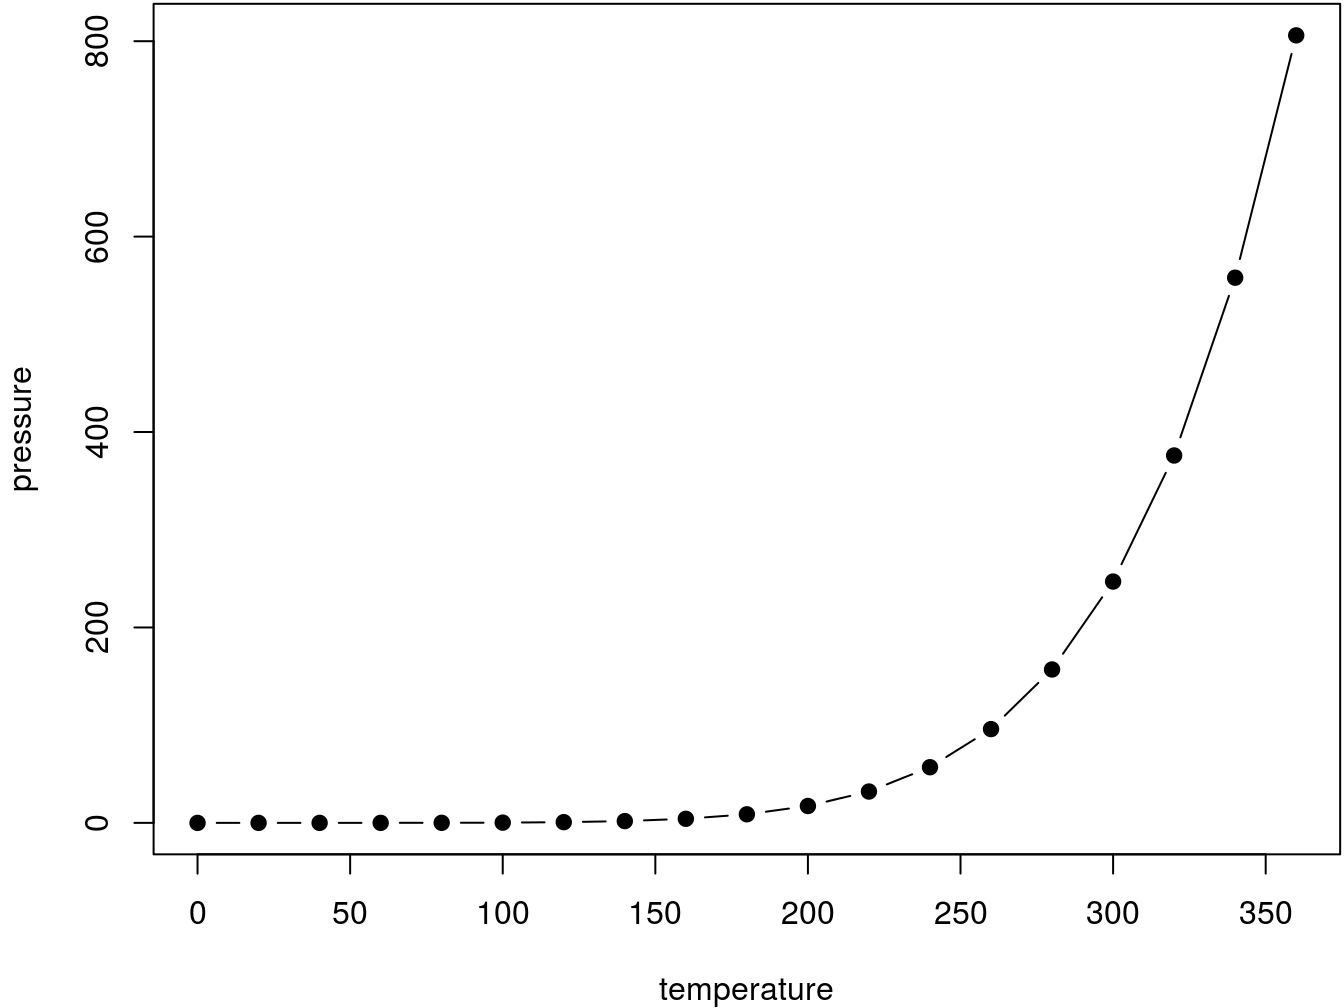
\includegraphics[width=0.8\linewidth]{math697_files/figure-latex/nice-fig-1} 

}

\caption{Here is a nice figure!}\label{fig:nice-fig}
\end{figure}

Reference a figure by its code chunk label with the \texttt{fig:}
prefix, e.g., see Figure \ref{fig:nice-fig}. Similarly, you can
reference tables generated from \texttt{knitr::kable()}, e.g., see Table
\ref{tab:nice-tab}.

\begin{Shaded}
\begin{Highlighting}[]
\NormalTok{knitr}\OperatorTok{::}\KeywordTok{kable}\NormalTok{(}
  \KeywordTok{head}\NormalTok{(iris, }\DecValTok{20}\NormalTok{), }\DataTypeTok{caption =} \StringTok{'Here is a nice table!'}\NormalTok{,}
  \DataTypeTok{booktabs =} \OtherTok{TRUE}
\NormalTok{)}
\end{Highlighting}
\end{Shaded}

\begin{table}

\caption{\label{tab:nice-tab}Here is a nice table!}
\centering
\begin{tabular}[t]{rrrrl}
\toprule
Sepal.Length & Sepal.Width & Petal.Length & Petal.Width & Species\\
\midrule
5.1 & 3.5 & 1.4 & 0.2 & setosa\\
4.9 & 3.0 & 1.4 & 0.2 & setosa\\
4.7 & 3.2 & 1.3 & 0.2 & setosa\\
4.6 & 3.1 & 1.5 & 0.2 & setosa\\
5.0 & 3.6 & 1.4 & 0.2 & setosa\\
\addlinespace
5.4 & 3.9 & 1.7 & 0.4 & setosa\\
4.6 & 3.4 & 1.4 & 0.3 & setosa\\
5.0 & 3.4 & 1.5 & 0.2 & setosa\\
4.4 & 2.9 & 1.4 & 0.2 & setosa\\
4.9 & 3.1 & 1.5 & 0.1 & setosa\\
\addlinespace
5.4 & 3.7 & 1.5 & 0.2 & setosa\\
4.8 & 3.4 & 1.6 & 0.2 & setosa\\
4.8 & 3.0 & 1.4 & 0.1 & setosa\\
4.3 & 3.0 & 1.1 & 0.1 & setosa\\
5.8 & 4.0 & 1.2 & 0.2 & setosa\\
\addlinespace
5.7 & 4.4 & 1.5 & 0.4 & setosa\\
5.4 & 3.9 & 1.3 & 0.4 & setosa\\
5.1 & 3.5 & 1.4 & 0.3 & setosa\\
5.7 & 3.8 & 1.7 & 0.3 & setosa\\
5.1 & 3.8 & 1.5 & 0.3 & setosa\\
\bottomrule
\end{tabular}
\end{table}

You can write citations, too. For example, we are using the
\textbf{bookdown} package \citep{R-bookdown} in this sample book, which
was built on top of R Markdown and \textbf{knitr} \citep{xie2015}.

\BeginKnitrBlock{rmdnote}
R is free software and comes with ABSOLUTELY NO WARRANTY. You are
welcome to redistribute it under the terms of the GNU General Public
License versions 2 or 3. For more information about these matters see
\url{http://www.gnu.org/licenses/}.
\EndKnitrBlock{rmdnote}

\begin{equation} 
  f\left(k\right) = \binom{n}{k} p^k\left(1-p\right)^{n-k}
  \label{eq:binom}
\end{equation}

See \eqref{eq:binom}

\BeginKnitrBlock{proof}
\iffalse <span class="proof"><em>Proof. \fi{} The characteristic
function of \(X\sim\mathrm{Pois}(\lambda)\) is
\(\varphi _{X}(t)=e^{\lambda (e^{it}-1)}\). Let \(P_n=\sum_{i=1}^nX_i\).
We know from Theorem \ref{thm:chf-sum} that

\begin{equation*}
\begin{split}
\varphi _{P_{n}}(t) & =\prod_{i=1}^n\varphi _{X_i}(t) \\
& =\prod_{i=1}^n e^{\lambda_i (e^{it}-1)} \\
& = e^{\sum_{i=1}^n \lambda_i (e^{it}-1)}
\end{split}
\end{equation*}

This is the characteristic function of a Poisson random variable with
the parameter \(\lambda=\sum_{i=1}^n \lambda_i\). From Lemma
\ref{lem:chf-pdf}, we know the distribution of \(P_n\) is
\(\mathrm{Pois}(\sum_{i=1}^n\lambda_i)\).
\EndKnitrBlock{proof}

\BeginKnitrBlock{theorem}[Pythagorean theorem]
\protect\hypertarget{thm:pyth}{}{\label{thm:pyth} \iffalse (Pythagorean
theorem) \fi{} }For a right triangle, if \(c\) denotes the length of the
hypotenuse and \(a\) and \(b\) denote the lengths of the other two
sides, we have \[a^2 + b^2 = c^2\]
\EndKnitrBlock{theorem}

Theorem \ref{thm:pyth}

\chapter{Literature}\label{literature}

\BeginKnitrBlock{rmdcaution}
R is free software and comes with ABSOLUTELY NO WARRANTY. You are
welcome to redistribute it under the terms of the GNU General Public
License versions 2 or 3. For more information about these matters see
\url{http://www.gnu.org/licenses/}.
\EndKnitrBlock{rmdcaution}

\BeginKnitrBlock{rmdimportant}
R is free software and comes with ABSOLUTELY NO WARRANTY. You are
welcome to redistribute it under the terms of the GNU General Public
License versions 2 or 3. For more information about these matters see
\url{http://www.gnu.org/licenses/}.
\EndKnitrBlock{rmdimportant}

\BeginKnitrBlock{rmdtip}
R is free software and comes with ABSOLUTELY NO WARRANTY. You are
welcome to redistribute it under the terms of the GNU General Public
License versions 2 or 3. For more information about these matters see
\url{http://www.gnu.org/licenses/}.
\EndKnitrBlock{rmdtip}

\BeginKnitrBlock{rmdwarning}
R is free software and comes with ABSOLUTELY NO WARRANTY. You are
welcome to redistribute it under the terms of the GNU General Public
License versions 2 or 3. For more information about these matters see
\url{http://www.gnu.org/licenses/}.
\EndKnitrBlock{rmdwarning}

\part{Part II}\label{part-part-ii}

\chapter{Methods}\label{methods}

\BeginKnitrBlock{example}[Example theorem]
\protect\hypertarget{ex:unnamed-chunk-5}{}{\label{ex:unnamed-chunk-5}
\iffalse (Example theorem) \fi{} }For a right triangle, if \(c\) denotes
the length of the hypotenuse and \(a\) and \(b\) denote the lengths of
the other two sides, we have \[a^2 + b^2 = c^2\]
\EndKnitrBlock{example}

\chapter{Applications}\label{applications}

Some \emph{significant} applications are demonstrated in this chapter.

\section{Example one}\label{example-one}

\section{Example two}\label{example-two}

\appendix


\chapter{Vectorization, *apply and for
loops}\label{vectorization-apply-and-for-loops}

This section will cover the basics of vectorizations, the
\texttt{*apply} family of functions and \texttt{for} loops.

\section{Vectorization}\label{vectorization}

Almost everything in \texttt{R} is a vector. A scalar is really a vector
of length 1 and a \texttt{data.frame} is a collection of vectors. An
nice feature of \texttt{R} is its vectorized capabilities. Vectorization
indicates that a function operates on a whole vector of values at the
same time and not just on a single value\footnote{\url{http://www.dummies.com/how-to/content/how-to-vectorize-your-functions-in-r.html}}.
If you have have ever taken a basic linear algebra course, this concept
will be familiar to you. \newline  \vspace{0.1in} Take for example two
vectors: \newline
\vspace{0.1in} \[
\begin{bmatrix} 1 \\ 2 \\ 3 \end{bmatrix} + 
\begin{bmatrix} 1 \\ 2 \\ 3 \end{bmatrix} =
\begin{bmatrix} 2 \\ 4 \\ 6 \end{bmatrix}
\] \newline  \vspace{0.1in} The corresponding \texttt{R} code is given
by:

\begin{Shaded}
\begin{Highlighting}[]
\NormalTok{a <-}\StringTok{ }\KeywordTok{c}\NormalTok{(}\DecValTok{1}\NormalTok{, }\DecValTok{2}\NormalTok{, }\DecValTok{3}\NormalTok{)}
\NormalTok{b <-}\StringTok{ }\KeywordTok{c}\NormalTok{(}\DecValTok{1}\NormalTok{, }\DecValTok{2}\NormalTok{, }\DecValTok{3}\NormalTok{)}
\NormalTok{a }\OperatorTok{+}\StringTok{ }\NormalTok{b}
\end{Highlighting}
\end{Shaded}

\begin{verbatim}
## [1] 2 4 6
\end{verbatim}

Many of the \texttt{base} functions in \texttt{R} are already
vectorized. Here are some common examples:

\begin{Shaded}
\begin{Highlighting}[]
\CommentTok{# generate a sequence of numbers from 1 to 10}
\NormalTok{(a <-}\StringTok{ }\DecValTok{1}\OperatorTok{:}\DecValTok{10}\NormalTok{)}
\end{Highlighting}
\end{Shaded}

\begin{verbatim}
##  [1]  1  2  3  4  5  6  7  8  9 10
\end{verbatim}

\begin{Shaded}
\begin{Highlighting}[]
\CommentTok{# sum the numbers from 1 to 10}
\KeywordTok{sum}\NormalTok{(a)}
\end{Highlighting}
\end{Shaded}

\begin{verbatim}
## [1] 55
\end{verbatim}

\begin{Shaded}
\begin{Highlighting}[]
\CommentTok{# calculate sums of each column}
\KeywordTok{colSums}\NormalTok{(iris[, }\OperatorTok{-}\DecValTok{5}\NormalTok{])}
\end{Highlighting}
\end{Shaded}

\begin{verbatim}
## Sepal.Length  Sepal.Width Petal.Length  Petal.Width 
##        876.5        458.6        563.7        179.9
\end{verbatim}

\begin{quote}
\textbf{Exercise}: What happens when you sum two vectors of different
lengths?
\end{quote}

\section{\texorpdfstring{Family of \texttt{*apply}
functions}{Family of *apply functions}}\label{family-of-apply-functions}

\begin{itemize}
\tightlist
\item
  \texttt{apply}, \texttt{lapply} and \texttt{sapply} are some of the
  most commonly used class of functions in \texttt{R}
\item
  \texttt{*apply} functions are not necessarily faster than loops, but
  can be easier to read (and vice cersa)
\item
  \texttt{apply} is used when you need to perform an operation on every
  row or column of a matrix or data.frame
\item
  \texttt{lapply} and \texttt{sapply} differ in the format of the
  output. The former returns a list while the ladder returns a vector
\item
  There are other \texttt{*apply} functions such as \texttt{tapply},
  \texttt{vapply} and \texttt{mapply} with similar functionality and
  purpose
\end{itemize}

\subsection{Loops vs.~Apply}\label{loops-vs.apply}

\begin{Shaded}
\begin{Highlighting}[]
\CommentTok{# Getting the row means of two columns Generate data}
\NormalTok{N <-}\StringTok{ }\DecValTok{10000}
\NormalTok{x1 <-}\StringTok{ }\KeywordTok{runif}\NormalTok{(N)}
\NormalTok{x2 <-}\StringTok{ }\KeywordTok{runif}\NormalTok{(N)}
\NormalTok{d <-}\StringTok{ }\KeywordTok{as.data.frame}\NormalTok{(}\KeywordTok{cbind}\NormalTok{(x1, x2))}
\KeywordTok{head}\NormalTok{(d)}
\end{Highlighting}
\end{Shaded}

\begin{verbatim}
##          x1         x2
## 1 0.1356226 0.21527199
## 2 0.2716021 0.26700884
## 3 0.4793413 0.53208314
## 4 0.7397965 0.05376706
## 5 0.3435368 0.53268188
## 6 0.4487223 0.01851926
\end{verbatim}

\begin{Shaded}
\begin{Highlighting}[]
\CommentTok{# Loop: create a vector to store the results in}
\NormalTok{rowMeanFor <-}\StringTok{ }\KeywordTok{vector}\NormalTok{(}\StringTok{"double"}\NormalTok{, N)}

\ControlFlowTok{for}\NormalTok{ (i }\ControlFlowTok{in} \KeywordTok{seq_len}\NormalTok{(N)) \{}
\NormalTok{    rowMeanFor[[i]] <-}\StringTok{ }\KeywordTok{mean}\NormalTok{(}\KeywordTok{c}\NormalTok{(d[i, }\DecValTok{1}\NormalTok{], d[i, }\DecValTok{2}\NormalTok{]))}
\NormalTok{\}}

\CommentTok{# Apply:}
\NormalTok{rowMeanApply <-}\StringTok{ }\KeywordTok{apply}\NormalTok{(d, }\DecValTok{1}\NormalTok{, mean)}

\CommentTok{# are the results equal}
\KeywordTok{all.equal}\NormalTok{(rowMeanFor, rowMeanApply)}
\end{Highlighting}
\end{Shaded}

\begin{verbatim}
## [1] TRUE
\end{verbatim}

\subsection{\texorpdfstring{Descriptive Statistics using
\texttt{*apply}}{Descriptive Statistics using *apply}}\label{descriptive-statistics-using-apply}

\begin{Shaded}
\begin{Highlighting}[]
\KeywordTok{data}\NormalTok{(women)}
\CommentTok{# data structure}
\KeywordTok{str}\NormalTok{(women)}
\end{Highlighting}
\end{Shaded}

\begin{verbatim}
## 'data.frame':    15 obs. of  2 variables:
##  $ height: num  58 59 60 61 62 63 64 65 66 67 ...
##  $ weight: num  115 117 120 123 126 129 132 135 139 142 ...
\end{verbatim}

\begin{Shaded}
\begin{Highlighting}[]
\CommentTok{# calculate the mean for each column}
\KeywordTok{apply}\NormalTok{(women, }\DecValTok{2}\NormalTok{, mean)}
\end{Highlighting}
\end{Shaded}

\begin{verbatim}
##   height   weight 
##  65.0000 136.7333
\end{verbatim}

\begin{Shaded}
\begin{Highlighting}[]
\CommentTok{# apply 'fivenum' function to each column}
\KeywordTok{vapply}\NormalTok{(women, fivenum, }\KeywordTok{c}\NormalTok{(}\DataTypeTok{Min. =} \DecValTok{0}\NormalTok{, }\StringTok{`}\DataTypeTok{1st Qu.}\StringTok{`}\NormalTok{ =}\StringTok{ }\DecValTok{0}\NormalTok{, }\DataTypeTok{Median =} \DecValTok{0}\NormalTok{, }\StringTok{`}\DataTypeTok{3rd Qu.}\StringTok{`}\NormalTok{ =}\StringTok{ }\DecValTok{0}\NormalTok{, }
    \DataTypeTok{Max. =} \DecValTok{0}\NormalTok{))}
\end{Highlighting}
\end{Shaded}

\begin{verbatim}
##         height weight
## Min.      58.0  115.0
## 1st Qu.   61.5  124.5
## Median    65.0  135.0
## 3rd Qu.   68.5  148.0
## Max.      72.0  164.0
\end{verbatim}

\subsection{\texorpdfstring{Creating new columns using
\texttt{sapply}}{Creating new columns using sapply}}\label{creating-new-columns-using-sapply}

You can apply a \emph{user defined function} to columns or the entire
data frame:

\begin{Shaded}
\begin{Highlighting}[]
\CommentTok{# the ouput of sapply is a vector the 's' in sapply stands for 'simplified'}
\CommentTok{# apply}
\NormalTok{mtcars}\OperatorTok{$}\NormalTok{gear2 <-}\StringTok{ }\KeywordTok{sapply}\NormalTok{(mtcars}\OperatorTok{$}\NormalTok{gear, }\ControlFlowTok{function}\NormalTok{(i) }\ControlFlowTok{if}\NormalTok{ (i }\OperatorTok{==}\StringTok{ }\DecValTok{4}\NormalTok{) }\StringTok{"alot"} \ControlFlowTok{else} \StringTok{"some"}\NormalTok{)}

\KeywordTok{head}\NormalTok{(mtcars)[, }\KeywordTok{c}\NormalTok{(}\StringTok{"gear"}\NormalTok{, }\StringTok{"gear2"}\NormalTok{)]}
\end{Highlighting}
\end{Shaded}

\begin{verbatim}
##                   gear gear2
## Mazda RX4            4  alot
## Mazda RX4 Wag        4  alot
## Datsun 710           4  alot
## Hornet 4 Drive       3  some
## Hornet Sportabout    3  some
## Valiant              3  some
\end{verbatim}

\subsection{\texorpdfstring{Applying functions to subsets using
\texttt{tapply}}{Applying functions to subsets using tapply}}\label{applying-functions-to-subsets-using-tapply}

\begin{Shaded}
\begin{Highlighting}[]
\CommentTok{# Fisher's famous dataset}
\KeywordTok{data}\NormalTok{(iris)}
\KeywordTok{str}\NormalTok{(iris)}
\end{Highlighting}
\end{Shaded}

\begin{verbatim}
## 'data.frame':    150 obs. of  5 variables:
##  $ Sepal.Length: num  5.1 4.9 4.7 4.6 5 5.4 4.6 5 4.4 4.9 ...
##  $ Sepal.Width : num  3.5 3 3.2 3.1 3.6 3.9 3.4 3.4 2.9 3.1 ...
##  $ Petal.Length: num  1.4 1.4 1.3 1.5 1.4 1.7 1.4 1.5 1.4 1.5 ...
##  $ Petal.Width : num  0.2 0.2 0.2 0.2 0.2 0.4 0.3 0.2 0.2 0.1 ...
##  $ Species     : Factor w/ 3 levels "setosa","versicolor",..: 1 1 1 1 1 1 1 1 1 1 ...
\end{verbatim}

\begin{Shaded}
\begin{Highlighting}[]
\CommentTok{# mean sepal length by species}
\KeywordTok{tapply}\NormalTok{(iris}\OperatorTok{$}\NormalTok{Sepal.Length, iris}\OperatorTok{$}\NormalTok{Species, mean)}
\end{Highlighting}
\end{Shaded}

\begin{verbatim}
##     setosa versicolor  virginica 
##      5.006      5.936      6.588
\end{verbatim}

\subsection{\texorpdfstring{Nested for loops using
\texttt{mapply}}{Nested for loops using mapply}}\label{nested-for-loops-using-mapply}

\texttt{mapply} is my favorite \texttt{base} \texttt{R} function and
here are some reasons why:

\begin{itemize}
\tightlist
\item
  Using \texttt{mapply} is equivalent to writing nested \texttt{for}
  loops except that it is 100\% more human readable and less prone to
  errors
\item
  It is an effective way of conducting simulations because it iterates
  of many arguments
\end{itemize}

Let's say you want to generate random samples from a normal distribution
with varying means and standard deviations. Of course the brute force
way would be to write out the command once, copy paste as many times as
you want, and then manually change the arguments for \texttt{mean} and
\texttt{sd} in the \texttt{rnorm} function as so:

\begin{Shaded}
\begin{Highlighting}[]
\NormalTok{v1 <-}\StringTok{ }\KeywordTok{rnorm}\NormalTok{(}\DecValTok{100}\NormalTok{, }\DataTypeTok{mean =} \DecValTok{5}\NormalTok{, }\DataTypeTok{sd =} \DecValTok{1}\NormalTok{)}
\NormalTok{v2 <-}\StringTok{ }\KeywordTok{rnorm}\NormalTok{(}\DecValTok{100}\NormalTok{, }\DataTypeTok{mean =} \DecValTok{10}\NormalTok{, }\DataTypeTok{sd =} \DecValTok{5}\NormalTok{)}
\NormalTok{v3 <-}\StringTok{ }\KeywordTok{rnorm}\NormalTok{(}\DecValTok{100}\NormalTok{, }\DataTypeTok{mean =} \OperatorTok{-}\DecValTok{3}\NormalTok{, }\DataTypeTok{sd =} \DecValTok{10}\NormalTok{)}
\end{Highlighting}
\end{Shaded}

This isn't too bad for three vectors. But what if you want to generate
many more combinations of means and sds ? Furthermore, how can you keep
track of the parameters you used? Now lets consider the \texttt{mapply}
function:

\begin{Shaded}
\begin{Highlighting}[]
\NormalTok{means <-}\StringTok{ }\KeywordTok{c}\NormalTok{(}\DecValTok{5}\NormalTok{, }\DecValTok{10}\NormalTok{, }\OperatorTok{-}\DecValTok{3}\NormalTok{)}
\NormalTok{sds <-}\StringTok{ }\KeywordTok{c}\NormalTok{(}\DecValTok{1}\NormalTok{, }\DecValTok{5}\NormalTok{, }\DecValTok{10}\NormalTok{)}

\CommentTok{# MoreArgs is a list of arguments that dont change}
\NormalTok{randomNormals <-}\StringTok{ }\KeywordTok{mapply}\NormalTok{(rnorm, }\DataTypeTok{mean =}\NormalTok{ means, }\DataTypeTok{sd =}\NormalTok{ sds, }\DataTypeTok{MoreArgs =} \KeywordTok{list}\NormalTok{(}\DataTypeTok{n =} \DecValTok{100}\NormalTok{))}

\KeywordTok{head}\NormalTok{(randomNormals)}
\end{Highlighting}
\end{Shaded}

\begin{verbatim}
##          [,1]      [,2]      [,3]
## [1,] 5.851127 16.981559 -1.995026
## [2,] 3.613288 15.208544  7.608420
## [3,] 3.705362  6.663188  7.639518
## [4,] 6.304945 11.361456 -7.565889
## [5,] 5.267800 10.431325  3.637958
## [6,] 5.588270  7.622221  5.763472
\end{verbatim}

The following diagram (from
\href{http://r4ds.had.co.nz/iteration.html\#mapping-over-multiple-arguments}{r4ds})
describes exactly what is going on in the above function call to
\texttt{mapply}:

\begin{figure}
\centering
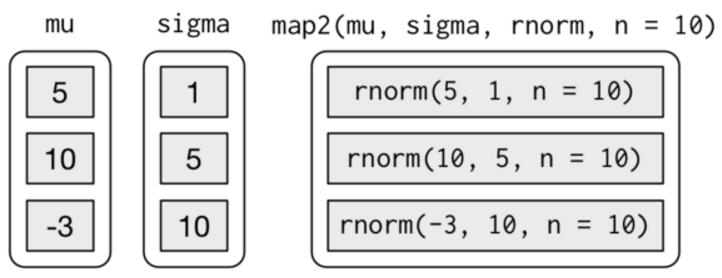
\includegraphics{images/mapply.png}
\caption{}
\end{figure}

Advantages:

\begin{enumerate}
\def\labelenumi{\arabic{enumi}.}
\tightlist
\item
  Result is automatically stored in a matrix
\item
  The parameters are also saved in \texttt{R} objects so that they can
  be easily manipulated and/or recovered
\end{enumerate}

Consider a more complex scenario where you want to consider many
possible combinations of means and sds. We take advantage of the
\texttt{expand.grid} function to create a \texttt{data.frame} of
simulation parameters:

\begin{Shaded}
\begin{Highlighting}[]
\NormalTok{simParams <-}\StringTok{ }\KeywordTok{expand.grid}\NormalTok{(}\DataTypeTok{means =} \DecValTok{1}\OperatorTok{:}\DecValTok{10}\NormalTok{, }\DataTypeTok{sds =} \DecValTok{1}\OperatorTok{:}\DecValTok{10}\NormalTok{)}

\NormalTok{randomNormals <-}\StringTok{ }\KeywordTok{mapply}\NormalTok{(rnorm, }\DataTypeTok{mean =}\NormalTok{ simParams}\OperatorTok{$}\NormalTok{means, }\DataTypeTok{sd =}\NormalTok{ simParams}\OperatorTok{$}\NormalTok{sds, }\DataTypeTok{MoreArgs =} \KeywordTok{list}\NormalTok{(}\DataTypeTok{n =} \DecValTok{100}\NormalTok{))}

\KeywordTok{dim}\NormalTok{(randomNormals)}
\end{Highlighting}
\end{Shaded}

\begin{verbatim}
## [1] 100 100
\end{verbatim}

\section{\texorpdfstring{Creating dynamic documents with
\texttt{mapply}}{Creating dynamic documents with mapply}}\label{creating-dynamic-documents-with-mapply}

\texttt{mapply} together with the \texttt{rmarkdown} package
\citep{R-rmarkdown} can be very useful to create dynamic documents for
exploratory analysis. We illustrate this using the Motor Trend Car Road
Tests data which comes pre-loaded in \texttt{R}.

\begin{quote}
The data was extracted from the 1974 Motor Trend US magazine, and
comprises fuel consumption and 10 aspects of automobile design and
performance for 32 automobiles (1973--74 models).
\end{quote}

Copy the code below in a file called \texttt{mapplyRmarkdown.Rmd} :

Copy the code below in a file called \texttt{boxplotTemplate} :

\chapter{Appendix B}\label{appendix-b}

\bibliography{packages.bib,book.bib}


\end{document}
